%% Time-stamp: <2019-02-01 09:10:32 (marc)>
\documentclass[xcolor=x11names,compress, mathserif]{beamer}

\newcommand\hmmax{0}
\newcommand\bmmax{0}

\usepackage{../includes/MarkMathCmds}

\newcommand{\hackspace}{\hspace{4.2mm}}
\newcommand{\showstudent}[1]{}





% talk/author information
\newcommand{\authorname}{Mark van der Wilk}
\newcommand{\authoremail}{m.vdwilk@imperial.ac.uk}
\newcommand{\authoraffiliation}{
 Department of Computing\\Imperial
  College London}
\newcommand{\authortwitter}{markvanderwilk}
\newcommand{\slidesettitle}{\imperialBlue{Sampling \& Monte Carlo}}
\newcommand{\footertitle}{Logistic Regression}
\newcommand{\location}{Imperial College London}
\newcommand{\talkDate}{{February 20, 2023}}


\date{\imperialGray{\talkDate}}




% load defaults
\input{../includes/header.tex}
\input{../includes/titlepage.tex}

\linespread{1.2}


\begin{frame}{Previously on Probabilistic Inference}
  We looked at \emph{logistic regression}
  \begin{itemize}
  \item Different kind of data (binary classification)
  \item Different assumptions in model
  \end{itemize}

  \vspace{0.5cm} \pause

  We wanted to
  \begin{itemize}
  \item Make predictions
  \item Find posterior
  \end{itemize} \pause
  Both computations were \emph{intractable}.
\end{frame}




\section{Monte Carlo Estimation}



\begin{frame}{Numerical Quadrature}
  Intractable computation are caused by \emph{integrals}.
  \begin{align}
    p(y^*\given x^*, \vy, X) &= \int p(y^*\given x^*, \vtheta)p(\vtheta\given \vy, X) \calcd{\vtheta} \\
    p(\vtheta\given \vy, X) &= \frac{p(\vy\given X, \vtheta)p(\vtheta)}{p(\vy\given X)} = \frac{p(\vy\given X, \vtheta)p(\vtheta)}{\int p(\vy\given X, \vtheta)p(\vtheta) \calcd{\vtheta}}
  \end{align}

  \pause
  Can we approximate numerically? \pause Evaluate on a \emph{grid}.

  \begin{figure}
    \centering Rectangle rule \hspace{0.23cm}
    \includegraphics[width=0.6\hsize,trim=0 1.2cm 0 0,clip]{./figures/mcmc/int-rect} \\
    \vspace{-0.2cm}
    Trapezoidal rule
    \includegraphics[width=0.6\hsize]{./figures/mcmc/int-trap}
  \end{figure}
\end{frame}




\begin{frame}{Numerical Quadrature in High Dimensions}
  We may have many parameters! For linear / logistic regression:
  \begin{itemize}
  \item $\vtheta \in \Reals^D$
  \item Even more if we use basis functions!
  \item  It is very common to have $> 100$ parameters
  \end{itemize}
  
  \pause
  \vspace{0.4cm}

For $D$ dimensions, there are $P^D$ total points in the grid. For $P\!=\!10$, $D\!=\!100$, that is more than the number of atoms in the universe.

\pause
\begin{itemize}
  \item \emph{Rate} of convergence depends on dimension (e.g.~$O(P_{\text{total}}^{-\frac{1}{D}})$ for rectangle rule)
  \item Need exponential number of points with dimension \\ \pause
  to reduce error by a factor of 2, you need $P_2/P_1 = 2^D$
\end{itemize}
\pause
\begin{center}
\Large \emph{Curse of Dimensionality}
\end{center}
\end{frame}




\begin{frame}{Monte Carlo Approximation}
Most Bayesian computations are in fact \emph{expectations}

E.g.~prediction for logistic regression
\begin{align}
p(y^*\given x^*, \vy, X) &= \int p(y^*\given x^*, \vtheta)p(\vtheta\given \vy, X) \calcd{\vtheta} \\
&= \Exp{p(\vtheta\given \vy, X)}{p(y^*\given x^*, \vtheta)} \,.
\end{align}

\pause

In general,
\begin{align}
I &= \Exp{p(\vx)}{g(\vx)} \\
\implies I &\approx \hat{I} = \frac{1}{S}\sum_{s=1}^S g(\vx^{(s)}) \,, & \text{with } \vx^{(s)} \stackrel{\text{iid}}{\sim} p(\vx) \,.
\end{align}

\end{frame}



\begin{frame}{Monte Carlo Properties}
Monte Carlo estimator
\begin{itemize}
\item mean is equal to the quantity we want to estimate (\emph{unbiased})
\begin{align}
\Exp{p(\vx^{(1)}, \vx^{(2)}, \dots)}{\hat{I}} = \int \prod_{t=1}^Sp(\vx^{(t)}) \frac{1}{S}\sum_{s=1}^Sg(\vx^{(s)}) \calcd{\{\vx^{(u)}\}_{u=1}^S} = I
\end{align}
(Bring sum outside, distributions for $s\neq t$ integrate to 1) \pause
\item variance decreases \emph{independent of dimension}
\begin{align}
\Var{p(\vx^{(1)}, \vx^{(2)}, \dots)}{\hat{I}} = \frac{1}{S^2} \sum_{s=1}^S \Var{p(\vx)}{g(\vx)} = \frac{C}{S}
\end{align}
i.e.~error decreases as $O(\frac{1}{\sqrt{S}})$.
\end{itemize}
\end{frame}


\section{Monte Carlo with Exact Sampling}



\begin{frame}{How to generate samples}
When specifying a Monte Carlo approximation, you need a procedure for \emph{generating samples} from your distribution of interest $p(\vx)$.
\begin{itemize}
  \item Some distributions are easy to sample from (e.g.~Uniform, Standard Gaussian). You may assume that such samples are available in the exam.
  \item Often though, no direct procedure for sampling $p(\vx)$
\end{itemize}

\pause

\vspace{0.5cm}

Different procedures are have different sampling properties. Distributions can be
\begin{itemize}
\item easy to sample, hard to evaluate (GANs, VAEs),
\item easy to evaluate, hard to sample.
\end{itemize}
\end{frame}



\begin{frame}
\frametitle{Sampling Discrete Variables}
\begin{figure}
\centering
\includegraphics[width = 0.8\hsize]{./figures/mcmc/uniform_sampling}
\end{figure}


\begin{itemize}
\item $u\sim \mathcal{U}[0,1]$, where $\mathcal U$ is the uniform
  distribution
\item $u = 0.55 \Rightarrow x = c$
\end{itemize}
\end{frame}



% %%%%%%%%%%%%%%%%%%%%%%%%%%%%%%%%%%%%%%%%%%%%%%%%%%%%%%


\begin{frame}
\frametitle{Continuous Variables}

\begin{figure}
\centering
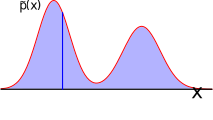
\includegraphics[height = 4cm]{./figures/mcmc/uniform_under_curve.pdf}
\end{figure}
\vspace{-0.5cm}
\begin{align}
P(z_1 < Z < z_2) = \int_{z_1}^{z_2} p(z) \calcd{z}
\end{align}

Geometric intuition: sample uniformly from the area under the curve
\end{frame}



\begin{frame}
\frametitle{Sampling Continuous Values}

Let's convert samples from  $\mathcal U [0,1]$ to samples from
densities
\vspace{-0.3cm}
\begin{columns}
\column{0.5\hsize}
\begin{figure}
\includegraphics[height = 5cm]{./figures/mcmc/inverse_transform_sampling}
\end{figure}
\column{0.5\hsize}

Objective: Sample from $p(y)$.

\begin{itemize}
\item $h(y) = \int_{-\infty}^y p(z) dz$ (CDF)
\item Draw $u\sim \mathcal U[0,1]$
\item Obtain sample from $p(y)$: \newline $y(u) = h\inv(u)$
\end{itemize}
\arrow \cemph{Inverse Transform Sampling} \\[2mm]
\end{columns}
% \vspace{5mm}
\pause
\begin{itemize}
\item \calert{We cannot always invert the CDF $h(y)$} \\
\item \calert{Difficult for high-dimensional distributions}
\end{itemize}
\end{frame}





\begin{frame}
\frametitle{Rejection Sampling: Setting}

\begin{figure}
\centering
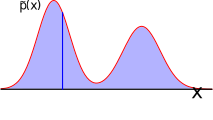
\includegraphics[height = 3cm]{./figures/mcmc/uniform_under_curve.pdf}
\end{figure}


\begin{itemize}
\item Assume:
\begin{itemize}
\item Sampling from $p(z)$ is difficult
\item Evaluating $\tilde p(z) = Zp(z)$ is easy (and $Z$ may be
  unknown)
\end{itemize}
\pause
\item Find a simpler distribution (\cemph{proposal distribution})
  $q(z)$ from which we can easily draw samples (e.g., Gaussian, Uniform)
\item Find an \cemph{upper bound} $kq(z)\geq \tilde p(z)$
\end{itemize}

\end{frame}




\begin{frame}
\frametitle{Rejection Sampling: Algorithm}
\begin{figure}
\centering
\includegraphics[]{./figures/mcmc/Figure11_4_annotated}\\
\tiny Adapted from PRML (Bishop, 2006)
\end{figure}
%
\begin{enumerate}
\item Generate $z_0\sim q(z)$
\item Generate $u_0\sim \mathcal U[0, kq(z_0)]$
%\item The pair $(z_0, u_0)$ is uniform under the curve of $kq(z)$. 
\item If $u_0 > \tilde p(z_0)$, reject the sample. Otherwise, retain $z_0$ 
\end{enumerate}
\end{frame}
%%%%%%%%%%%%%%%%%%%%%%%%%%%%%%%%%%%%%%% 

\begin{frame}
\frametitle{Properties}
%
\begin{figure}
\centering
\includegraphics[]{./figures/mcmc/Figure11_4_annotated}\\
\tiny Adapted from PRML (Bishop, 2006)
\end{figure}

\begin{itemize}
\item Accepted pairs $(z,u)$  are uniformly distributed under the curve of
$\tilde p(z)$
\item Marginal probability density of the $z$-coordiantes of accepted points
  must be proportional to $\tilde p(z)$
\item \cemph{Samples are independent samples from $p(z)$}
\end{itemize}
\end{frame}


%%%%%%%%%%%%%%%%%%%%%%%%%%%%%%%%%%%%%%%
\begin{frame}
\frametitle{Sampling in High Dimensions}

Example:
\begin{itemize}
\item $p(\vec x) = \gauss{\vec 0}{\sigma_p^2\mat I}$,\quad $q(\vec x) =
  \gauss{\vec 0}{\sigma_q^2\mat I}$ where $\sigma_q = 1.01\sigma_p$
\item What is the value of $k$ if $\vec x\in\R^{1000}$?
  \pause
\item $q(0) = 1/(2\pi\sigma_q^2)^{500}$ \arrow For $kq\geq p$ we need to
  set
\begin{align*}
k\geq \frac{p(0)}{q(0)} = \frac{(\sigma_q^2)^{500}}{(\sigma_p^2)^{500}} =
\exp\big(1000\ln\frac{\sigma_q}{\sigma_p}\big) = \exp(1000\ln
  1.01) \approx 20,000
\end{align*} \pause
\item \cemph{Acceptance rate} is the ratio of the volume under $p$ to the volume
  under $kq$. In our example: $1/k = 1/20,000$.
\end{itemize} \pause

\begin{itemize}
\item In high dimensions the factor $k$ is probably huge\\ \arrow \alert{Low
  acceptance rate}
\item Finding $k$ is tricky
\end{itemize}
\end{frame}


%%%%%%%%%%%%%%%%%%%%%%%%%%%%%%%%%%%%%%%
\begin{frame}
\frametitle{Shortcomings}

\begin{figure}
\centering
\includegraphics[]{./figures/mcmc/Figure11_4_annotated}\\
\tiny Adapted from PRML (Bishop, 2006)
\end{figure} \pause
\begin{itemize}[<+->]
\item Finding the upper bound $k$ is tricky
\item In high dimensions the factor $k$ is probably huge
\item \alert{Low acceptance rate/high rejection rate} of samples 
\end{itemize}
\end{frame}


% %%%%%%%%%%%%%%%%%%%%%%%%%%%%%%%%%%%%%%%
% \begin{frame}
% \frametitle{Acceptance Probability}

% Acceptance probability:
% \begin{align*}
% p(\text{accept}) &= \int \frac{\tilde p(z)}{kq(z)}q(z) dz\\
% &= \frac{1}{k}\int \tilde p(z) dz
% \end{align*}

% \end{frame}



\begin{frame}
\frametitle{Importance Sampling}
\textbf{Key idea:} Do not throw away all rejected samples, but give them lower
weight by rewriting the integral as an expectation under a simpler
distribution $q$ (\cemph{proposal distribution}):

\begin{align*}
\E_p[f(\vec x)] &= \int f(\vec x) p(\vec x) d\vec x \\
\onslide+<2->{&=\int f(\vec x) p(\vec x)
\blue{\frac{q(\vec x)}{q(\vec x)}}d\vec x}
\onslide+<3->{ = \int f(x) \frac{p(\vec x)}{\blue{q(\vec x)}} \blue{q(\vec x)}d\vec x\\}
\onslide+<4->{&= \E_q\left[f(\vec x) \frac{p(\vec x)}{q(\vec x)}\right]}
\end{align*}
\onslide+<5->{If we choose $q$ in a way that we can easily sample from it, we can
approximate this last expectation by Monte Carlo:
%
\begin{align*}
\E_q\left[f(\vec x)\frac{p(\vec x)}{q(\vec x)}\right]\approx
\frac{1}{S}\sum_{s=1}^S f(\vec x\idx{s})\red{\frac{p(\vec x\idx{s})}{q(\vec x\idx{s})}}
\onslide+<6->{= \frac{1}{S}\sum_{s=1}^S \red{w_s} f(\vec x{\idx{s}})},\quad \vec x\idx{s}\sim q(\vec x)
\end{align*}
}

\end{frame}


%%%%%%%%%%%%%%%%%%%%%%%%%%%%%%%%%%%%%%%%%%%%%%%%%%%%%%
\begin{frame}
\frametitle{Properties}

\begin{itemize}[<+->]
% \item Importance sampling estimator is \cemph{consistent}, but
%   \calert{biased}
\item Unbiased if $q>0$ where $p>0$ and if we can evaluate $p$
%\item No independent samples from the posterior
\item Breaks down if we do not have enough samples (puts nearly all
  weight on a single sample)\\ \arrow \calert{Degeneracy} (see also
  \cemph{Particle Filtering} (Thrun et al., 2005))
\item \calert{Many draws} from proposal density $q$ required,
  especially in high dimensions
\item Requires to be able to evaluate true $p$.  Generalization exists
  for $\tilde p$. This generalization is biased (but consistent).
\item Does not scale to interesting (high-dimensional) problems
\end{itemize}
\onslide+<6>{
\arrow Different approach to sample from complicated
(high-dimensional) distributions 
}
\end{frame}



\begin{frame}{Conclusion}
We saw:
\begin{itemize}
\item Why rectangle quadrature rules don't work in high dimensions
\item How Monte Carlo estimators help
\item How to draw samples using
\begin{itemize}
\item Transformation techniques
\item Inverse Transform Sampling
\item Rejection Sampling
\end{itemize}
\item How to improve over Rejection Sampling with Importance Sampling
\end{itemize}
\end{frame}


\begin{frame}{References}
\cite{itila}
\end{frame}








%%%%%%%%%%%%%%%%%%%%%%%%%%%%%%%%%%%%%%%%%
% REFERENCES
%%%%%%%%%%%%%%%%%%%%%%%%%%%%%%%%%%%%%%%%%
\begin{frame}[t,allowframebreaks]
\frametitle{References}
\linespread{1.0}
\tiny
\bibliographystyle{abbrv}
\bibliography{../includes/pi-literature}
\end{frame}



\end{document}
%%% Local Variables: 
%%% mode: latex
%%% TeX-master: t
%%% End: 
